
We describe  \sys's architecture and basic operation in Section~\ref{ssec:overview}.
We then discuss in-memory compaction policies  in  Section~\ref{ssec:policies}
and implementation details in Section~\ref{ssec:impl-details}. 

\subsection{Overview} \label{ssec:overview}

\begin{figure}[tbh]
\center
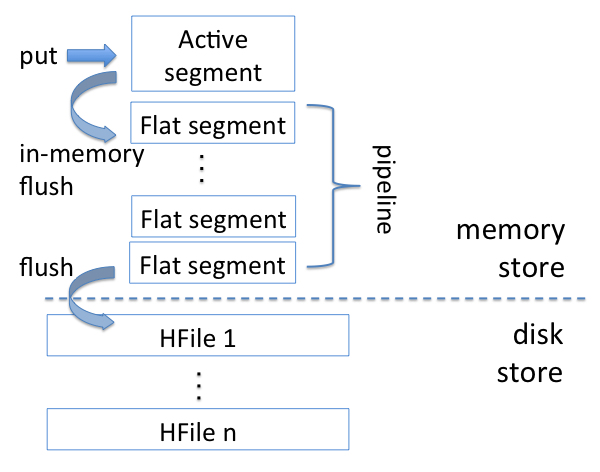
\includegraphics[width=\columnwidth, trim={0 1cm 0 1cm}, clip]{Accordion} 
\caption{Accordion's compacting memory store architecture. The memory store includes a small dynamic active segment 
and a pipeline of flat segments. }
\label{fig:accordion}
\end{figure}

\sys\ introduces a \emph{compacting} memory store to the LSM tree design framework. In contrast to the traditional memory store, 
which maintains RAM-resident data in a single monolithic data structure, \sys\ manages data as a \emph{pipeline} of 
\emph{segments} ordered by creation time. At all times, the most recent segment, called \emph{active}, is mutable;
it absorbs  put operations. The rest of the segments are immutable. Get and scan operations retrieve data from all  segments, 
 similarly to a traditional LSM tree read from multiple files. 
 
 Figure~\ref{fig:accordion} illustrates the \sys\ architecture. It is parameterized by two values:
\begin{itemize}
\item  $A$ -- the fraction of the memory store allocated to the active segment; and 
\item $S$ -- the upper bound on the number of immutable segments in the pipeline. 
\end{itemize}

\noindent
As our experiments show (Section~\ref{sec:eval}), the most effective parameter values are quite small -- 
(\inred{$0.02 \leq A \leq 0.05$}, and \inred{$1 \leq S \leq 3$}).

The memory store dynamics are as follows. 
Once the active segment grows to a $\rho$ fraction of the memory store's size bound, an \emph{in-memory flush} is invoked.
The flush makes the active segment  immutable and adds it to the pipeline; it creates a new active segment to replace it. 
Once the number of immutable segments exceeds $s$, a background \emph{in-memory compaction} is invoked to shrink
the pipeline back. It applies one or more mechanisms: 
\begin{enumerate}
\item {\em Flattening of intra-segment search indices.} Replaces dynamic segment indices such as skiplists by 
compact ordered arrays, which are suitable for immutable data. 
 \remove{ % Off-heap stuff omitted due to lack of evaluation
 % To Do: move to conclusions
 An additional advantage of the flat layout  is that in managed environments, 
the index can be relocated to off-heap (unmanaged) memory, which can improves performance predictability 
through reduced garbage collection jitter~\cite{alibabahbase}. 
}
\item {\em Merging multiple segments' search indices.} 
Replaces multiple segments with one by creating a single index covering data that resides 
in the original segments. This is a lightweight process that does not eliminate redundant 
data versions, and hence does not involve physical data copy. 
\item  {\em Merging multiple segments' data.} Extends the above with redundant data elimination --
creates a flat index with no redundancies, and disposes the redundant data cells. 
\remove{ % Slab stuff omitted due to lack of evaluation
In case the memstore manages its cell data storage internally, the surviving cells are relocated
to new slabs; otherwise, the redundant cells are simply de-referenced, and later garbage-collected.    
}
\end{enumerate} 
The choice of compaction mechanisms to employ is guided by the policies described in Section~\ref{ssec:policies}.

Flushes to disk work the same way as in a standard LSM tree. A disk flush freezes the list of immutable segments 
to be written to storage, and removes them from the pipeline. The background flush process merges the frozen 
segments while eliminating the redundancies, and streams the result to a new file. Note that the disk flush process
may happen concurrently to in-memory compaction. In that case, the latter is aborted. This behavior is absolutely
valid since in-memory compaction it is an optimization that may be retried later.

\subsection{Compaction Policies} \label{ssec:policies}

We implement three in-memory compaction policies: 
\begin{description}
\item[\basic] (low-overhead). Once a segment becomes immutable, flattens its index. Once the pipeline size exceeds $s$, 
merges all segment indices into one.  
\item[\eager] (high-overhead, high-reward under self-similar workloads). 
In addition to \basic\/ mechanisms, eliminates data redundancies in all pipeline segments.
\item[\adp] (the best of all worlds)\footnote{\small{Not committed to production code yet.}}. A heuristic that chooses 
whether to apply data compaction (as in \eager) or not (as in \basic) based on the level of redundancy in the data 
and the perceived cost-effectiveness of compaction. Works at store level, i.e., triggers redundancy elimination 
only for those stores where positive impact is expected. 
\end{description}

\adp\/ triggers in-memory compaction with probability $t$ if the fraction of redundant keys $r$ exceeds a parameter 
threshold $R$. In this context, $t$ is the throttling factor, which captures the compaction's worthiness. It starts from 
$T=0.5$, grows exponentially by $2\%$ with the number of in-memory flushes, and is reset back to $T$ upon
disk flush. The rationale is that compactions become more effective as the memory store grows bigger. 

$r$ is the complement of the ratio of unique keys in the memory store, denoted  $u$. The latter is approximated 
as a the fraction of unique keys produced by the process of merging the segment indexes during the previous compaction. 
Note that $u$ is an estimate, since compactions do not cover the current active segment. However, since the latter is a small 
portion of the memory store, the error is insignificant. 

\remove{
\begin{description}
\item[\emph{Unique ratio}] $u$ -- an estimate of the fraction of unique keys out of the total number of items in the segment. 
This value is estimated by counting duplicates encountered during merge, which does not induce extra overhead since
merged items are compared in any case. The \emph{unique\_ratio}  is an under-estimate of the actual redundancy because it does not 
take into consideration duplicates that were already present during flattening. Nevertheless, since the active component
is typically quite small, the error due to the under-estimate is significant only when the component is still small 
(has not undergone many merges), and compaction is therefore less important.
\item[\emph{success\_probability}] -- an estimate of the probability of a compaction yielding the expected benefits based on recent history.
Here, we define an expected space reduction threshold below which compaction is not cost-effective. 
We initialize the \emph{success\_probability} to some default value (e.g., $0.5$). 
Then, if compaction yields the expected benefit (i.e., frees up more space than the threshold) we increase the \emph{success\_probability},
and otherwise decrease it. The \emph{success\_probability} is reset to its default value upon flushes. 
The rationale for using \emph{success\_probability} is that its prediction becomes more accurate with time, whence 
compactions become more important because the component is bigger and more space can be saved.
\end{description}
}

\subsection{Implementation Details} \label{ssec:impl-details}

A compacting memstore is comprised from the active segment and a double-ended queue (pipeline) of inactive segments. 
The pipeline is accessed by read API's (get and scan), as well as by background disk flushes and in-memory compactions. 
The latter two modify the pipeline, by adding/removing/replacing segments. These modifications happen infrequently. 

The pipeline readers and writers coordinate through a lightweight copy-on-write, as follows. The pipeline object is versioned. 
Each modification promotes the version number, and atomically swaps the global reference to the new version clone. Note
that cloning is inexpensive -- only the segment references are copied since the segments themselves are immutable. 

The reads access the segments lock-free, through the version obtained at the beginning of the operation. If a disk flush
is scheduled in the middle of a read, a segment may migrate from the pipeline to the pre-flush snapshot buffer. The read 
safety is guaranteed by scanning the pipeline clone first. This way, a segment may be encountered twice but no data is 
lost. The scan algorithm filters out the duplicates. 

In-memory compaction is a read-modify-write operation, which swaps one or more segments in the pipeline 
with a new segment built from their data. This operation's atomicity is guaranteed by compare-and-swap (CAS), 
which flips pipeline version only if the latter did not change since the compaction started.  For example, in-memory
compaction fails if a disk flush concurrently removes some segments from the pipeline (Section~\ref{ssec:overview}). 

